\section{Question 8.4}


\subsection{Question}
For two queries in the CACM collection, generate two uninterpolated recall-precision graphs, a table of interpolated precision values at standard recall levels, and the average interpolated recall-precision graph.


\subsection{Approach}
Using the \texttt{getrel.py}, \texttt{q84.py} and \texttt{graphs.R} scripts, found in Listings \ref{listing:getrel}, \ref{listing:q84} and \ref{listing:graphsR}.


\lstinputlisting[language=Python, caption={The run function}, label=listing:runfunc,linerange={59-63},firstnumber=59]{code/getrel/getrel.py}


\subsubsection{Generating the Uninterpolated Recall-Precision Graph}
The generated graph is shown in Figure \ref{fig:urpgraph66}.

\begin{figure}[H]
\centering
\label{fig:urpgraph68}
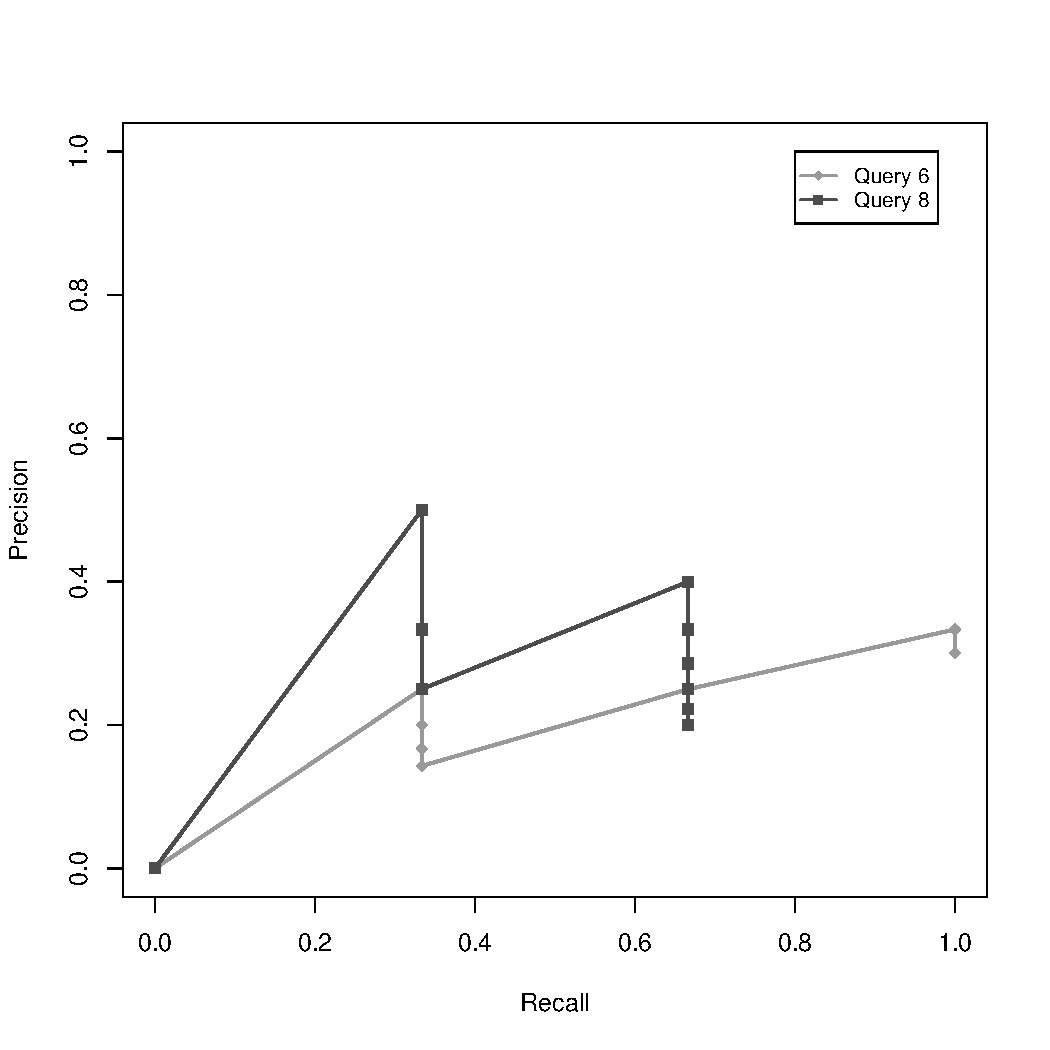
\includegraphics[scale=.6]{code/getrel/urpg68.pdf}
\caption{Uninterpolated Recall-Precision Graph for CACM Queries 6 and 8.}
\end{figure}


\subsubsection{Generating the Table of Interpolated Precision Values}



\subsubsection{Generating the Average Interpolated Recall-Precision Graph}

\begin{figure}[H]
\centering
\label{fig:aiprgraph68}
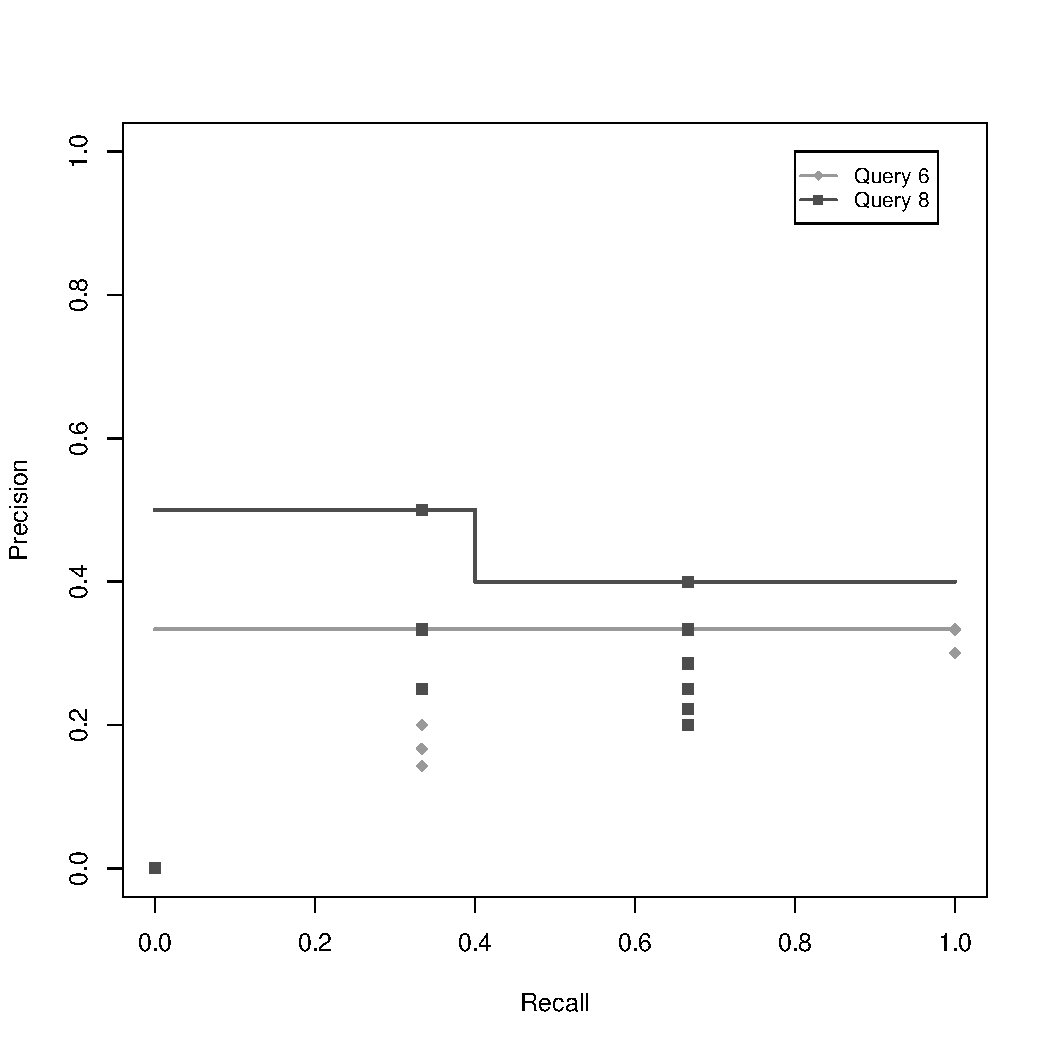
\includegraphics[scale=.6]{code/getrel/ipr68.pdf}
\caption{Average Interpolated Recall-Precision Graph for CACM Queries 6 and 8.}
\end{figure}




